
In the rest of this thesis, we present our approaches that contribute to achieve our goal: automatic non-functional testing and tuning of generators. Figure \ref{fig:overview} depicts an overview of how the different contributions we propose are connected to each other and how they contribute to address the challenges of the state of the art, described earlier.

\begin{figure}[h]
	\center
	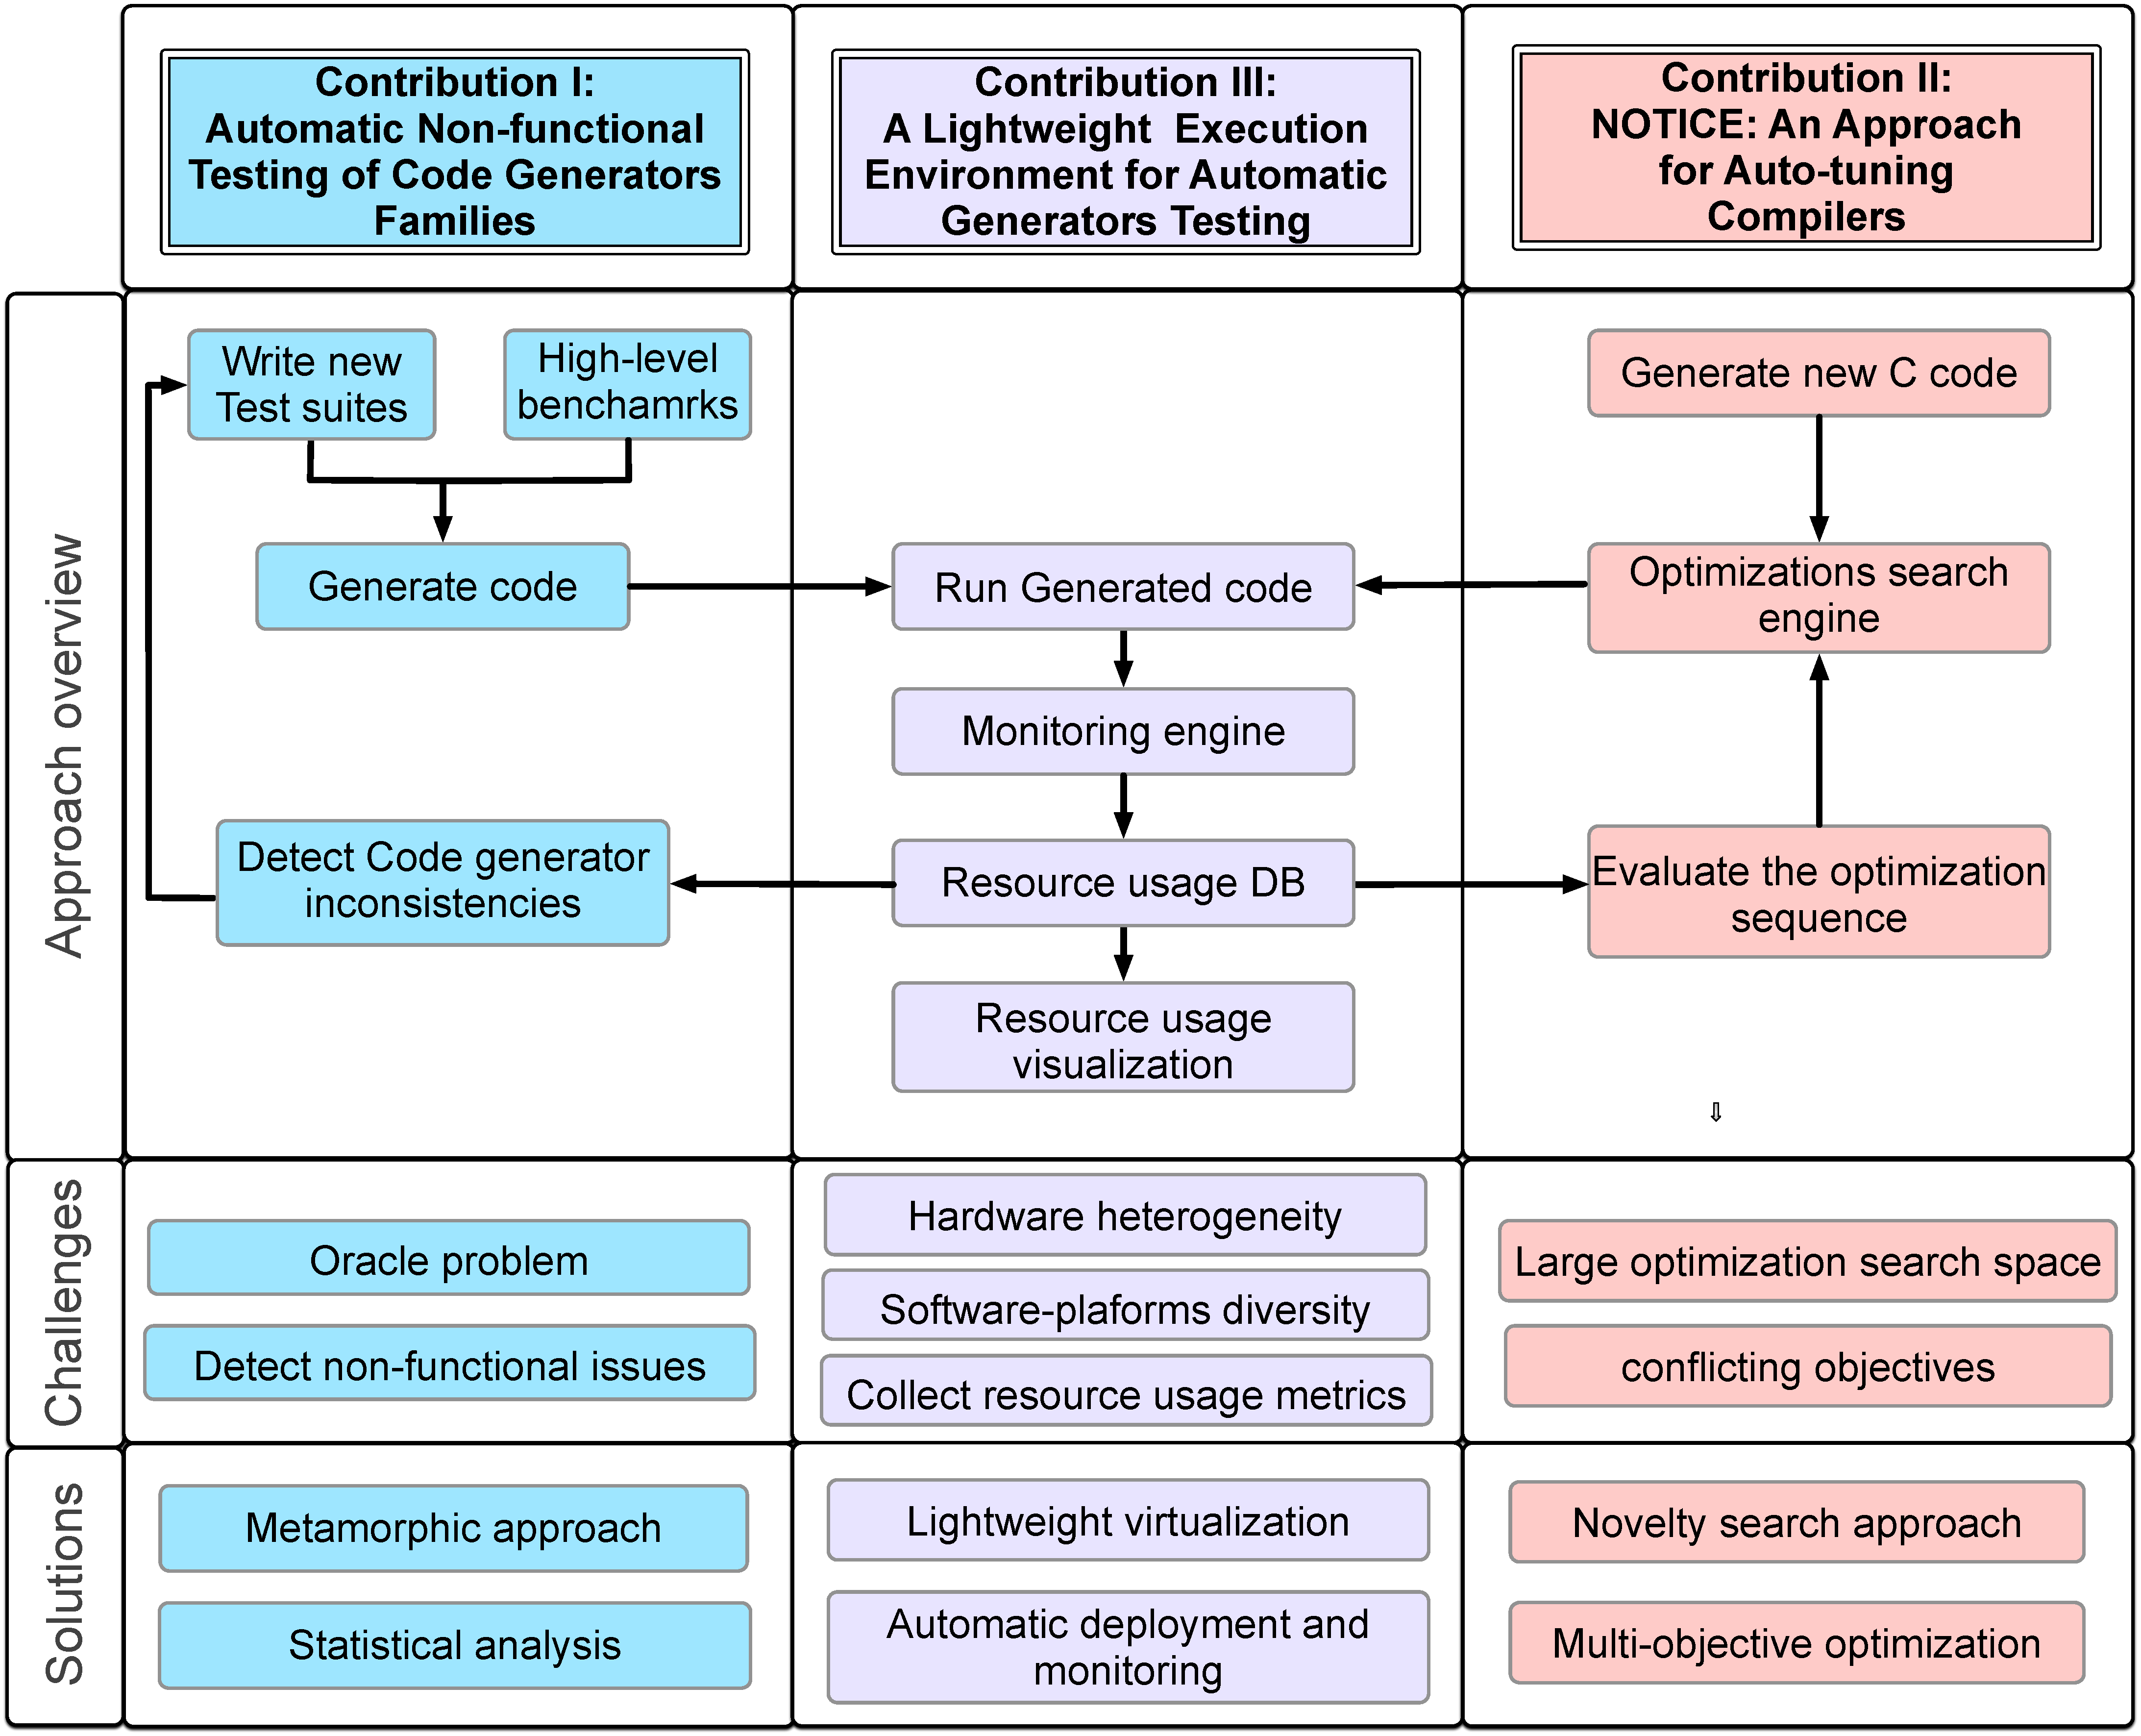
\includegraphics[scale=0.23]{Chapitre0/fig/overview}
	\caption{Summary of contributions}
	\label{fig:overview}
\end{figure}

This thesis makes three main contributions:
\begin{itemize}
	\item \textbf{Contribution I: Automatic non-functional testing of code generators families (in blue): }
	
	In this contribution (Chapter \ref{chap:code generators}), we propose an approach for automatic non-functional  testing of code generators. As discussed earlier, existing solutions lack of automation and efficiency to find code generator issues. Particularly, the oracle problem as well as the test of non-functional properties are not addressed. In this contribution, we address the limitations of the state of the art, describing an approach based on metamorphic testing and statistical analysis to efficiently detect inconsistencies within code generator families.
	Starting from a set of high-level benchmarks and test suites, we automatically generate source code to five target software platforms (\ie, using a code generator family). We execute the generated code and evaluate the resource usage metrics using the lightweight testing infrastructure presented in contribution III. Inconsistencies are then reported for further inspection.  
	
	\item \textbf{Contribution II: NOTICE, An approach for auto-tuning compilers (in red):}
	
	We address in this contribution two main problems: exploring the large optimization search space and finding trade-offs between conflicting objectives. 
	Thus, we present in Chapter \ref{chap:compilers}, an adaptation of the Novelty Search algorithm to the problem of compilers auto-tuning. Our contribution focuses on tuning GCC compilers based on randomly generated C programs.
	This approach shares the same monitoring infrastructure as the previous contribution in order to evaluate the impact of discovered optimization sequences on resource usage. The outcome of this approach is the best set of optimization options for a given hardware architecture, for a given input program, and for a specific non-functional property (\ie, execution time, CPU consumption, and memory usage). We also conduct a multi-objective optimization to tackle the problem of conflicting objectives (\eg, memory usage and execution time).
	
	\item \textbf{Contribution III: A lightweight execution environment for automatic generators testing (in purple):}
	
	We propose in Chapter \ref{chap:docker}, a common infrastructure used by both previous contributions to gather information about the quality of generated code in terms of memory and CPU usage. It serves as a lightweight execution environment to easily run tests across different software and hardware settings. In particular, it is based on micro-services, namely Docker, in order to automate software deployment, execution and monitoring. Finally, we provide a mechanism to visualize at runtime the resource consumption of running programs. This contribution addresses the limitations of the state of the art, namely the lack of solutions that handle the software and hardware diversity when testing/tuning generators.
\end{itemize}

The validation of each contribution is presented in the corresponding chapter. Different experiments are used to illustrate the characteristics of each solution we present.



